\chapter{Popis navrženého řešení a použitých technologií}


\section{Architektura navrženého řešení}


\begin{figure}[h]
\begin{centering}
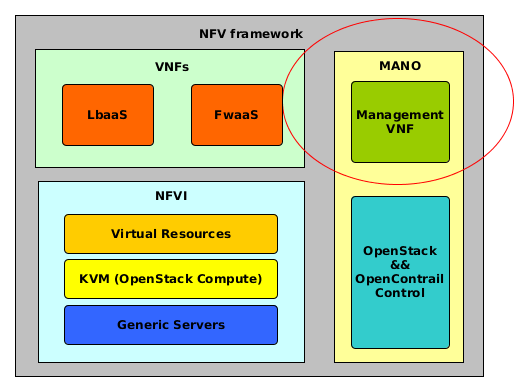
\includegraphics[scale=0.51]{images/VNF_overview}
\par\end{centering}
\caption{Architektura NFV řešení\label{fig:VNF_overview}}
\end{figure}


\section{OpenStack}\label{sub:interaction}

Popis Openstacku

OpenStack Heat Templates are used to demonstrate load balancing and firewalling inside of Openstack.

\section{OpenContrail}\label{sub:interaction}

Popis OpenContrailu.


\section{Heat Templates}


\begin{figure}[h]
\begin{centering}
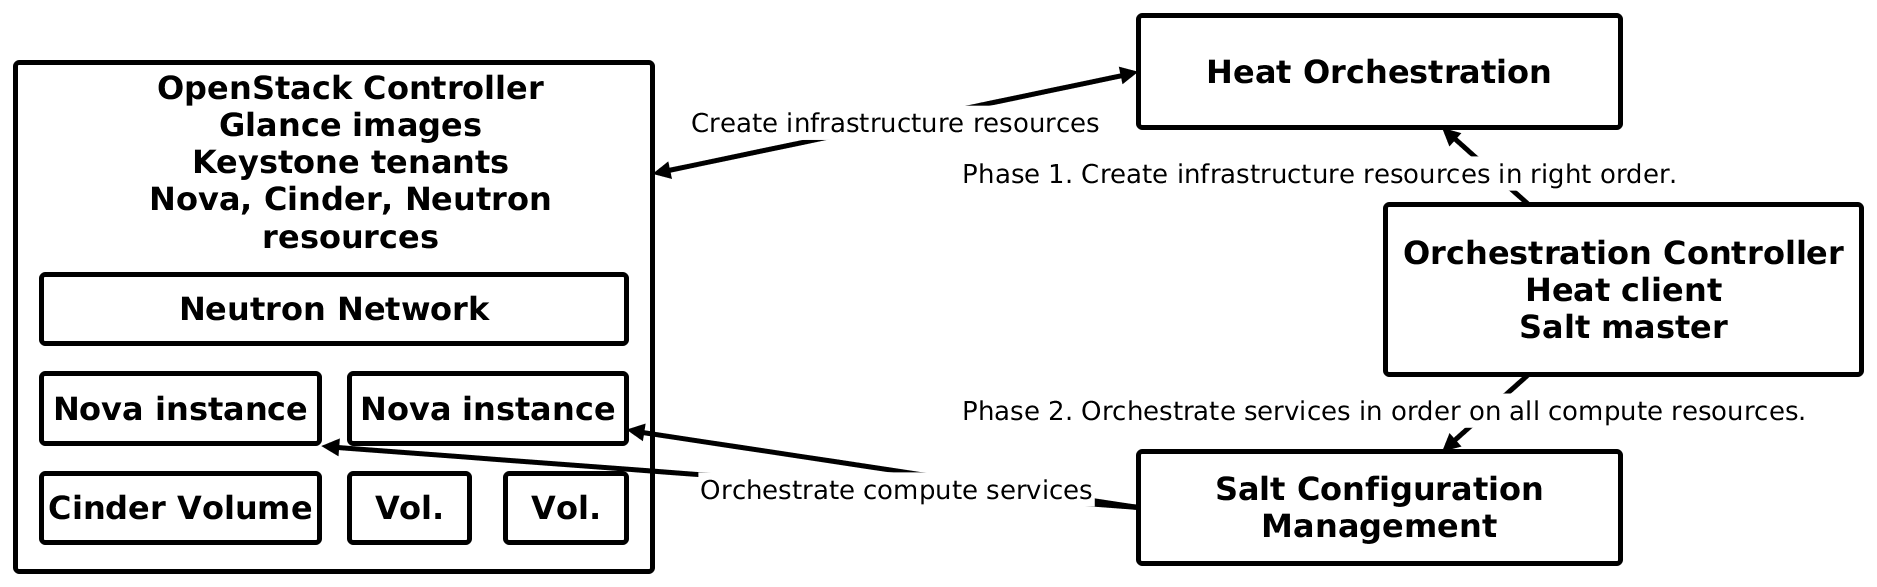
\includegraphics[scale=0.21]{images/heat}
\par\end{centering}
\caption{Popis heat orchestrace\label{fig:heat}}
\end{figure}

Popis co jsou to heat templates.

Heat is the main project of the OpenStack orchestration program. It allows users to describe deployments of complex cloud applications in text files called templates. These templates are then parsed and executed by the Heat engine.

\subsection{FwaaS template}

Pro FwaaS je narhnut heat template, který obsahuje:

\begin{itemize}
\item 1 firewall instanci
\item 1 testovaci instanci
\item 1 management instanci
\item management síť
\item privátní síť
\item contrail policy
\end{itemize}



\subsection{LbaaS template}


Navržený heat template pro LbaaS v sobě obsahuje následující prostředky, které se po spuštění pokusí vytvořit.

\begin{itemize}
\item pool
\item members
\item health monitoring
\item 2 web instance
\item privatni síť
\item public síť
\end{itemize}
